%%%%%%%%%%%%%%%%%%%%%%%%%%%%%%%%%%%%%%%%%%
\chapter{Desarrollo experimental} \label{chap:DesExp}
 En este capítulo se explicarán detalladamente el enfoque de investigación y la metodología empleada en el proyecto. Además, se detallará el diseño del sistema hidropónico de tipo DFT propuesto y los componentes utilizados en su implementación.
\section{Sistema hidropónico basado en la técnica de flujo profundo}

De acuerdo con la recopilación de información y la experiencia adquirida durante el desarrollo de este proyecto de investigación, se decidió utilizar un sistema hidropónico DFT por su alta eficiencia en el uso del agua, ya que, las raíces están constantemente en contacto con los nutrientes y el agua, reduciendo la evaporación y la pérdida de agua, permitiendo una absorción más efectiva de estos nutrientes por las raíces, lo que reduce el uso de más nutrientes y los costos asociados. Otro de sus beneficios es el espacio y densidad de plantación, ya que los sistemas DFT son adecuados para el cultivo en espacios reducidos debido a su diseño en capas horizontales. Esta disposición permite una mayor densidad de plantas por unidad de área, lo que es valioso en entornos con espacio limitado. En cuestión económica se reduce el consumo eléctrico, ya que la bomba de suministro se activa solo durante ciertos periodos, en comparación con otros sistemas, como el NFT o el vertical, en donde el funcionamiento de las bombas es constante.

Con base en la estructura básica de un sistema hidropónico de tipo DFT, se diseñó una estructura en el software SolidWorks con los siguientes materiales y medidas:
\begin{itemize}
\item Tubo de Policloruro de Vinilo (PVC, por sus siglas en inglés) de 3 pulgadas. 
\item Tapas de 3 pulgadas.
\item Conexiones tipo T de 3 pulgadas.
\item Conexiones tipo codo de 3 pulgadas.
\item Tubo hidráulico de 1 pulgada.
\item Tapas de 1 pulgada.
\item Conexiones tipo T de 1 pulgadas.
\item Conexiones tipo codo de 1 pulgadas.
\item Conexiones tipo Macho-Hembra de 1 pulgadas.
\item Llave de paso de 1 pulgada.
\item Tuvo flexible de 1 pulgada.
\item Pegamento Adhesivo para PVC.
\item Canastillas hidropónicas.
\item Bomba eléctrica periférica para agua 1/2 Hp.
\end{itemize}

El sistema hidropónico de tipo DFT se creó mediante una estructura de tubos de PVC de diferentes medidas. Los tubos del sistema donde se encuentran las plantas son 8 tubos de 3 pulgadas con una longitud de 1.5 metros, donde la separación entre los tubos era de 22 centímetros. Utilizando la misma separación, se realizaron 5 o 6 barrenos de 2 pulgadas y un barreno de 1.5 pulgadas en la sección de alimentación de agua entre los tubos. Cada una de las medidas permiten usar todo el espacio para sembrar, mientras que la forma rectangular de la instalación, permite utilizar codos y conexiones de tubería tipo T de PVC estándar. La parte del sistema DFT que contiene la estructura de los canales de riego y siembra se muestra en la figura \ref{sistema1}.

Para la etapa de alimentación del sistema DFT se utilizó una bomba de agua periférica eléctrica de 1 pulgada y 1/2 caballo de fuerza. La potencia de la bomba se seleccionó en forma experimental y se verificó que genera el caudal necesario para  el sistema. Para conectar la bomba se usó tubería hidráulica de 1 pulgada, utilizando conexiones tipo T y llaves de paso para regular el flujo de agua entre los canales de riego. Además, se agregó una salida de retorno en la bomba para mejorar la oxigenación de la solución nutritiva. Los dibujos en software CAD del sistema de alimentación se muestran en la figura \ref{sistema2}. La unión de la estructura de los canales de riego y la etapa de alimentación hidráulica del sistema DFT se muestran en la figura \ref{sistema3}.

 \begin{figure}[H]
\centering
         \includegraphics[scale=0.8]{imgs/1.8m.png} \\
    \caption{Diseño de la estructura de los canales de riego y siembra en SolidWorks. }\label{sistema1}
\end{figure}
\newpage
 \begin{figure}[H]
\centering
         \includegraphics[scale=0.8]{imgs/alimentacion.PNG} \\
    \caption{Diseño del sistema de alimentación en SolidWorks. }\label{sistema2}
\end{figure}
 \begin{figure}[H]
\centering
         \includegraphics[scale=0.75]{imgs/diseño.PNG} \\
    \caption{Diseño del sistema hidropónico DFT propuesto con 8 canales de riego. }\label{sistema3}
\end{figure}

De manera complementaria, se realizó un diseño de dos canales de riego con el fin de realizar una estimación inicial de los precios de construcción y efectuar la experimentación inicial. Este diseño se muestra en la figura \ref{sistema2Canales}
 \begin{figure}[H]
\centering
         \includegraphics[scale=0.65]{imgs/1.2.png} \\
    \caption{Diseño del sistema hidropónico DFT propuesto con 2 canales de riego. }\label{sistema2Canales}
\end{figure}

\section{Monitoreo de variables}
Dentro de un ciclo de cosecha en un sistema hidropónico es necesario mantener estables ciertas condiciones a su alrededor, las cuales varían de acuerdo a las estaciones del año y el lugar donde se encuentra instalado el sistema. Un controlador automático permite mantener estables las variables de importancia para el crecimiento de las plantas en un sistema hidropónico sin prácticamente intervención humana. Las variables principales que influyen en el crecimiento de las plantas en un sistema hidropónico se describen a continuación.

\subsection{Potencial de hidrógeno (pH)}

El pH del líquido en un sistema hidropónico es un factor crítico para el crecimiento y la salud de las plantas. El pH se refiere al grado de acidez o alcalinidad del líquido en el que se cultivan las plantas y puede tener un impacto significativo en la absorción de nutrientes y la salud general de las plantas. Si el pH del líquido es demasiado alto (alcalino), puede causar la deficiencia de nutrientes. Además, puede provocar que las hojas de las plantas se vuelvan amarillas y se caigan. Por otro lado, si el pH del líquido es demasiado bajo (ácido), puede causar la decoloración de las hojas y el crecimiento deficiente de las raíces. Por lo tanto, es importante mantener el pH del líquido dentro de un rango óptimo para el crecimiento y la salud de las plantas. El rango de pH óptimo puede variar según el tipo de planta cultivada, pero generalmente se encuentra entre 6 y 8. Por ende, se implementará un control automático dentro de la solución nutritiva \cite{singh2016electrical}.

\subsection{Conductividad eléctrica}
La conductividad eléctrica en un sistema hidropónico se refiere a la capacidad del líquido para conducir electricidad. En técnicas hidropónicas, la conductividad eléctrica del líquido es un indicador importante de la cantidad de nutrientes disueltos en el agua. La conductividad eléctrica se mide en unidades de partes por millón ($ppm$), milisiemens por centímetro ($mS/cm$) o bien microsiemens por centímetro ($\mu S/cm$) . La conductividad eléctrica en un sistema hidropónico debe estar dentro de un rango específico para garantizar el crecimiento y la salud de las plantas. Si la conductividad eléctrica es demasiado alta, puede indicar que hay demasiados nutrientes disueltos en el agua y esto puede dañar las raíces de las plantas. Por otro lado, si la conductividad eléctrica es demasiado baja, puede indicar que las plantas no están recibiendo suficientes nutrientes. El rango de conductividad eléctrica óptima en un sistema hidropónico varía según el tipo de planta cultivada. En general, la conductividad eléctrica para plantas en la etapa de crecimiento vegetativo debe estar entre 1500 y 3000 $\mu S/cm$. Así mismo, se diseña un control automático en la solución nutritiva \cite{carrasco2007efecto}.

\subsection{Temperatura líquida}

En este tipo de sistemas, la temperatura del líquido en el que se cultivan las plantas es un factor crítico para el crecimiento y la salud de ellas.
\\
La temperatura del líquido de un sistema hidropónico puede afectar el crecimiento y la salud de las plantas de varias maneras. Por ejemplo, si la temperatura del líquido es demasiado alta, puede provocar la muerte de las raíces de las plantas y reducir la absorción de nutrientes. Por otro lado, si la temperatura del líquido es demasiado baja, puede reducir la tasa de crecimiento de las plantas y aumentar el riesgo de enfermedades. Es importante mantener la temperatura del líquido de un sistema hidropónico dentro de un rango óptimo para el crecimiento y la salud de las plantas \cite{carrasco2007efecto}.

\subsection{Humedad en el ambiente}
La humedad en el ambiente dentro de un sistema hidropónico también es un factor importante. La humedad en el ambiente se refiere a la cantidad de vapor de agua presente en el aire, y puede afectar la absorción de nutrientes y el crecimiento de las plantas. Si la humedad en el ambiente es demasiado baja, las plantas pueden experimentar estrés hídrico y tener dificultades para absorber suficientes nutrientes, lo que puede conducir a un crecimiento lento y a hojas marchitas. Por otro lado, si la humedad en el ambiente es demasiado alta, puede promover el crecimiento de hongos y bacterias que pueden afectar negativamente la salud de las plantas \cite{siddiq2019achpa}.

\section{Circuito de control}
Dentro de esta sección, se describe el diseño del circuito de control en el sistema, el cual utiliza los dispositivos eléctricos y electrónicos descritos en la tabla \ref{tab:componentes}.
\begin{table}[htb!]
\centering
\caption{Lista de componentes dentro del circuito de control. } 
\begin{tabular}{|p{2.8cm}|c|p{11.5cm}|}
\hline
      Componente & Cantidad & Descripción  \\
\noalign{\hrule height 2pt}
        Microcontrolador ESP32 & 1   & Es un microcontrolador de bajo costo con un procesador de doble núcleo de 32 bits, con conectividad Wi-Fi y Bluetooth. \\
        \hline
        Raspberry PI 3 B+ &  1 & Es una mini-computadora de bajo costo y alto rendimiento, diseñada para trabajar con sistemas operativos basados en Linux. \\
       \hline
     Sensor DHT11 &  1 & Sensor de temperatura y humedad con un rango de medición de temperatura entre 0°C y 50°C, y de humedad de 20 – 90\%. \\
     \hline
     Sensor PH-4502C & 1 & Es un dispositivo que permite medir el pH con ayuda de una sonda (electrodo E201). Su rango de detección es de 0-14 (ácido /base).\\
     \hline
     Sensor TDS meter v1 &  1 & Es un dispositivo que permite medir la CE por medio de un electrodo, detectando los iones conductivos en agua. Su rango de detección es de 0-1000 partes por millón. En esta tesis se utiliza como unidad de medida para la CE los microsiemens/centímetro $(\mu S/cm)$, con una equivalencia de $2 \mu S/cm = 1ppm$.\\
      \hline
        Sensor DS18B20 &   1 & Es un sensor digital de temperatura que utiliza el protocolo 1-Wire para comunicarse, con un rango de detección entre -55°C y 125°C.\\
         \hline
         Driver Puente H L298N & 2   & Es un circuito de control de motores mediante modulación por ancho de pulso (PWM, por sus siglas en inglés).\\
          \hline
          Módulo relevador de 2 canales & 1 & Es un interruptor electrónico que puede ser accionado mediante pulsos digitales. \\
           \hline
   Bombas peristálticas & 4 &   Es un elemento hidráulico que permite el desplazamiento de distintos tipos de fluidos. Estos fluidos son contenidos en un tubo flexible en forma de ``C'' dentro una pareja de rodillos aprietan el tubo flexible, y mediante un movimiento de rotación van trasegando el fluido.\\
    \hline
    \hline
\end{tabular}
\label{tab:componentes}
\end{table}

\newpage
El microcontrolador ESP32 está conectado con todos los actuadores y sensores del sistema para realizar los siguientes procesos:
\begin{itemize}
\item El control de las bombas peristálticas, las cuales suministran los nutrientes para el control del pH y conductividad eléctrica en la solución nutritiva. 
\item El encendido y apagado de la bomba periférica, la cual suministra la solución nutritiva en el sistema.
\item El encendido y apagado de la minilavadora, la cual se encarga de mezclar y generar oxigenación en la solución nutritiva.

\end{itemize}

Para la conexión inalámbrica se utiliza una Raspberry Pi 3 modelo B+ y el microcontrolador ESP32, el cual recibe los datos de los sensores y los envía por WiFi al \textit{broker} instalado en la Raspberry Pi. Los datos que envía son los generados por los sensores analógicos de pH, de temperatura del agua, humedad en el ambiente y conductividad eléctrica de la solución nutritiva.

En la figura \ref{circuito1} se muestra una representación gráfica del esquema de conexiones del circuito de control, incluyendo sensores y actuadores.
\begin{figure}[H]
\centering
         \includegraphics[scale=0.56, angle=90]{imgs/circuito.PNG} \\
    \caption{Esquema de conexiones del circuito de control.}\label{circuito1}
\end{figure}

\section{Control difuso para la dosificación de nutrientes}
Dentro de la investigación se ha planteado utilizar un controlador basado en lógica difusa, que permite manejar la incertidumbre y la vaguedad de los datos, lo que resulta especialmente adecuado para sistemas hidropónicos. Uno de los aspectos destacados de la utilización del control difuso, es su capacidad para adaptarse y ajustar automáticamente dadas las condiciones del sistema en respuesta a los cambios que sufra. Al optimizar automáticamente las condiciones del sistema, el control difuso puede reducir el desperdicio de agua y nutrientes al adaptarse continuamente a las necesidades de las plantas. Siendo un impacto positivo en la sustentabilidad, además ayuda en los costos operativos a largo plazo. Por lo cual, a continuación se describen los pasos realizados, para el desarrollo de un control difuso para la dosificación de nutrientes. Para la creación del controlador se utilizaron las 4 etapas vistas dentro de la investigación. 

\subsection{Parámetros previos}
En la primera etapa se deben tener en cuenta las entradas y salidas del sistema, ya que con ellas se construyen los antecedentes y consecuentes de las reglas de inferencia y se generan los universos de discurso dentro de los valores de referencia en el sistema. Estos valores se obtienen con base en el análisis de los límites de funcionamiento del sistema.
\begin{itemize}
    \item \textbf{Entradas.} La entrada del controlador es el error calculado mediante la diferencia entre el valor actual y el valor obtenido de los sensores de pH y CE. 
    \item \textbf{Salidas.} La salida del controlador es una señal de PWM generada por el microcontrolador ESP32, la cual será proporcional el voltaje de alimentación de las bombas peristálticas y está expresado en porcentaje.
    \item \textbf{Semántica de las entradas y salidas.} La semántica de las entradas y salidas se realiza utilizando las funciones de membresía, las cuales representarán los términos lingüísticos. Estas funciones pueden ser por ejemplo, triangulares, trapezoidales, sigmoidales o en forma campana generalizada. En la implementación desarrollada en esta tesis  se utilizan funciones lineales triangulares (Tri) y trapezoidales (Trap) debido a que son más simples de programar y requieren menos operaciones computacionales, lo que las hace ideales para su implementación en microcontroladores o procesadores embebidos, como el ESP32.
\end{itemize}

\subsection{Fusificación} En esta etapa se evalúan las funciones lineales propuestas para el error utilizando el mecanismo de inferencia difuso.
\newpage
\textbf{El universo de discurso del error de pH está en un rango de} [-14.0,14.0]

\textbf{Términos lingüísticos de entrada y salida sobre el pH:}

Se emplean 5 términos lingüísticos para el error con las siguientes funciones de membresía:
\begin{itemize}
 \item Error Negativo Grande (ENG, Trap) $\longrightarrow$ Rango (-14.0,-14.0,-9.0,-4.5)
 \item Error Negativo Pequeño (ENP, Tri) $\longrightarrow$ Rango (-9.0,-4.5,0.0)
 \item Error Cero (EC, Trap) $\longrightarrow$ Rango (-4.5,-1.5,1.5,4.5)
 \item Error Positivo Pequeño (EPP, Tri) $\longrightarrow$ Rango (0.0,4.5,9.0)  
 \item Error Positivo Grande (EPG, Trap) $\longrightarrow$ Rango (4.5,9.0,14.0,14.0)
 \end{itemize}

Para la salida sus 5 términos lingüísticos para el PWM son:
\begin{itemize}
 \item PWM Negativo Grande (PWMNG, Trap) $\longrightarrow$Rango (-100.0,-100.0,-50.0,-25.0)
 \item PWM Negativo Pequeño (PWMNP, Tri) $\longrightarrow$ Rango (-50.0,-25.0,0.0)
 \item PWM Cero (PWMC, Tri) $\longrightarrow$ Rango (-25.0,0.0,25.0)
 \item PWM Positivo Pequeño (PWMPP, Tri) $\longrightarrow$ Rango (0.0,25.0,50.0) 
 \item PWM Positivo Grande (PWMPG, Trap) $\longrightarrow$ Rango (25.0,50.0,100.0,100.0)
\end{itemize}

Las gráficas de las funciones de membresía del pH se observan en la figura \ref{ph1}.

\begin{figure}[H]
\centering
         \includegraphics[scale=0.75]{imgs/FuncionPH_Esp.png} \\
    \caption{Funciones de membresía de entrada y salida del pH.}\label{ph1}
\end{figure}

\textbf{Universo de discurso del error de la CE:} Error=[-4000.0,4000.0]

\textbf{Términos lingüísticos de entrada y salida sobre la CE:}

Se emplean 5 términos lingüísticos para el error sobre la CE:
\begin{itemize}
   
 \item Error Negativo Grande (ENG, Trap) $\longrightarrow$ Rango (-4000.0,-4000.0,-2915.0,-1835.0)
 \item Error Negativo Pequeño (ENP, Tri) $\longrightarrow$ Rango (-3670.0,-1835.0,0.0)
 \item Error Cero (EC, Trap) $\longrightarrow$ Rango (-1835.0,-750.0,750.0,1835.0)
 \item Error Positivo Pequeño (EPP, Tri) $\longrightarrow$ Rango (0.0,1835.0,3670.0)  
 \item Error Positivo Grande (EPG, Trap) $\longrightarrow$ Rango (1835.0,2915.0,4000.0,4000.0)
 \end{itemize}
 
Para la salida, los 5 términos lingüísticos usados para el PWM son:
\begin{itemize}
 \item PWM Negativo Grande (PWMNG, Trap) $\longrightarrow$ Rango (-100.0,-100.0,-50.0,-25.0)
 \item PWM Negativo Pequeño (PWMNP, Tri) $\longrightarrow$ Rango (-50.0,-25.0,0.0)
 \item PWM Cero (PWMC, Tri) $\longrightarrow$ Rango (-25.0,0.0,25.0)
 \item PWM Positivo Pequeño (PWMPP, Tri) $\longrightarrow$ Rango (0.0,25.0,50.0) 
 \item PWM Positivo Grande (PWMPG, Trap) $\longrightarrow$ Rango (25.0,50.0,100.0,100.0)
\end{itemize}

Las gráficas de las funciones de membresía de la CE se muestran en la figura \ref{conduc1}.

\begin{figure}[H]
\centering
         \includegraphics[scale=0.72]{imgs/FuncionCE_Esp.png} \\
    \caption{Funciones de membresía de entrada y salida de la conductividad eléctrica.}\label{conduc1}
\end{figure}


\subsection{Mecanismo de inferencia y reglas de inferencia} Para esta etapa se utiliza el método \textit{Modus Ponens} difuso, utilizado para evaluar reglas de tipo SI-ENTONCES, que son establecidas por un experto, para realizar conclusiones parciales. Las reglas generadas para el sistema se muestran en la tabla \ref{tab:t4}.\\
\begin{table}[H]
\centering
\caption{Reglas: Conclusiones parciales.} 
\begin{tabular}{ c c}
\textbf{Antecedente} & \textbf{Consecuente}\\
\hline
Si ENG & entonces PWMNG\\
Si ENP &entonces PWMNP\\
Si EC &entonces PWMC\\
Si EPP &entonces PWMPP\\
Si EPG &entonces PWMPG\\
\hline
\end{tabular}
\label{tab:t4}
\end{table}
Para cada sensor se establecieron las mismas reglas de la tabla \ref{tab:t4}. Las conclusiones parciales se estiman mediante la operación de disyunción, la cual es calculada mediante el mínimo de los valores de las funciones de membresía de las reglas difusas. Para generar la conclusión completa del controlador se usa la operación de unión de las conclusiones parciales, calculada mediante el máximo de las funciones de membresía correspondientes a las conclusiones parciales.

\subsection{Defusificación}
Para obtener la curva de control del sistema, se utiliza el método del centroide (COG), el cual es calculado mediante la ecuación \ref{eq:cog}.
\begin{equation}
    \label{eq:cog}
    COG=\frac{\int M(x)\cdot xdx}{\int M(x)dx},
\end{equation}
donde, $M(x)$ representa el grado de membresía del elemento $x$ que tomará valores en el universo de discurso, usando un paso definido por el usuario. Con este método se obtiene la salida del controlador, la cual es un porcentaje de PWM enviado a un driver de que genera el voltaje necesario para las bombas peristálticas de acuerdo con los niveles medidos de la variable observada en la solución nutritiva.

\section{Monitoreo remoto de un sistema DFT}
Para el monitoreo remoto se usan herramientas del IoT, que permiten visualizar parámetros de importancia en un sistema hidropónico adquiridos mediante los sensores colocados en el sistema. Se configuró el \textit{broker} Mosquitto en una computadora embebida Raspberry Pi, el cual usa el protocolo de mensajería MQTT. Este \textit{broker}, gestiona la suscripción y publicación de datos en tópicos en tiempo real. Los tópicos están asociados a los 4 sensores instalados en el sistema hidropónico. Los sensores envían las lecturas a un microcontrolador ESP32, el cual mediante una conexión WiFi, publica los datos recabados a \textit{broker}, el cual los almacena en una base de datos. Los datos almacenados pueden ser visualizados en forma gráfica, tanto en una aplicación móvil como una aplicación web vinculada a la plataforma Node-Red.

\textbf{Aplicación móvil.} Para la creación de la aplicación móvil se diseñó un nuevo servidor para el sistema como se observa en la figura \ref{app_1}.

\begin{figure}[H]
\centering
         \includegraphics[scale=0.45]{imgs/APP_2.png} \\
    \caption{Creación del servidor en la aplicación móvil.}\label{app_1}
\end{figure}
Después se configura dicho servidor con el \textit{broker} Mosquitto utilizando su IP como se aprecia en la figura \ref{app_2}. 
\begin{figure}[H]
\centering
         \includegraphics[scale=0.45]{imgs/APP_3.png} \\
    \caption{Configuración del IP con el \textit{broker}.}\label{app_2}
\end{figure}

Teniendo esto, se configuran los paneles deseados respecto a los valores que se obtendrán en la salida del controlador y de los sensores, en este caso se utilizan 4 paneles, estos se aprecian en la figura \ref{app_3}.

\begin{figure}[H]
\centering
         \includegraphics[scale=0.45]{imgs/APP_4.png} \\
    \caption{Configuración de paneles.}\label{app_3}
\end{figure}

\textbf{Servidor Node-Red.} Para la creación del servidor se realizó las mismas configuraciones creando un nuevo servidor enlazado con el \textit{broker} como se muestra en la figura \ref{Node_1} y en la figura \ref{Node_2} se aprecia la creación del servidor colocando los 4 paneles utilizados e información de enlace en el sistema.

\begin{figure}[H]
\centering
         \includegraphics[scale=0.5]{imgs/NODE-RED.png} \\
    \caption{Configuración de paneles.}\label{Node_1}
\end{figure}

\begin{figure}[H]
\centering
         \includegraphics[scale=0.55]{imgs/NODE-RED_2.png} \\
    \caption{Visualización del servidor.}\label{Node_2}
\end{figure}

\section{Monitoreo de germinación}
Para el monitoreo de la germinación de las plantas se usaron tres plantas herbáceas: 
\begin{itemize}
    \item Acelga
    \item Chile serrano
    \item Cilantro
\end{itemize}

Las semillas de estas plantas fueron plantadas dentro de una combinación de sustratos:
\begin{itemize}
    \item 1/4 de Vermiculita exfoliada. Este es un sustrato inerte ligero, con un pH neutro que favorece la buena aireación, aumenta la reflexión de la luz y absorbe grandes cantidades de agua.

    \item 1/4 de Perlita. Este sustrato blanco contiene un alto porcentaje de silicio, el cual ayuda a retener la humedad, protege del calor y ayuda a enraizar.
    \item 2/4 de tierra negra. Este es el sustrato más común en los plantíos debido a su capacidad natural de retener suficiente agua para el desarrollo de las plantas.
\end{itemize}

Una fotografía de los sustratos utilizados se puede observar en la figura \ref{sustratos}.
 \begin{figure}[!ht]
\centering
         \includegraphics[scale=0.15]{imgs/sustrato.jpeg} \\
    \caption{Sustratos empleados en la germinación. }\label{sustratos}
\end{figure}
\newpage

Las plantas fueron sometidas a 3 métodos diferentes de germinación:

\begin{itemize}
    \item\textbf{Método 1:} Es el método clásico de germinación, en el cual se colocan dentro de los semilleros las semillas y el sustrato, suministrando agua y una solución nutritiva en forma constante.
    \item \textbf{Método 2:} Es un método en el que se usa un recipiente profundo en el cual se colocan las semillas directamente en una solución nutritiva.
    \item \textbf{Método 3:} En este método se coloca un sustrato previamente humedecido en solución nutritiva y se coloca en los semilleros, donde se vuelve a humedecer, para después cubrirlo con un manto húmedo que lo protege del exterior y dejarlo reposar por 3 días.
\end{itemize}

El crecimiento inicial de las plantas en los semilleros se muestra en la figura \ref{plantas}.
 \begin{figure}[!ht]
\centering
         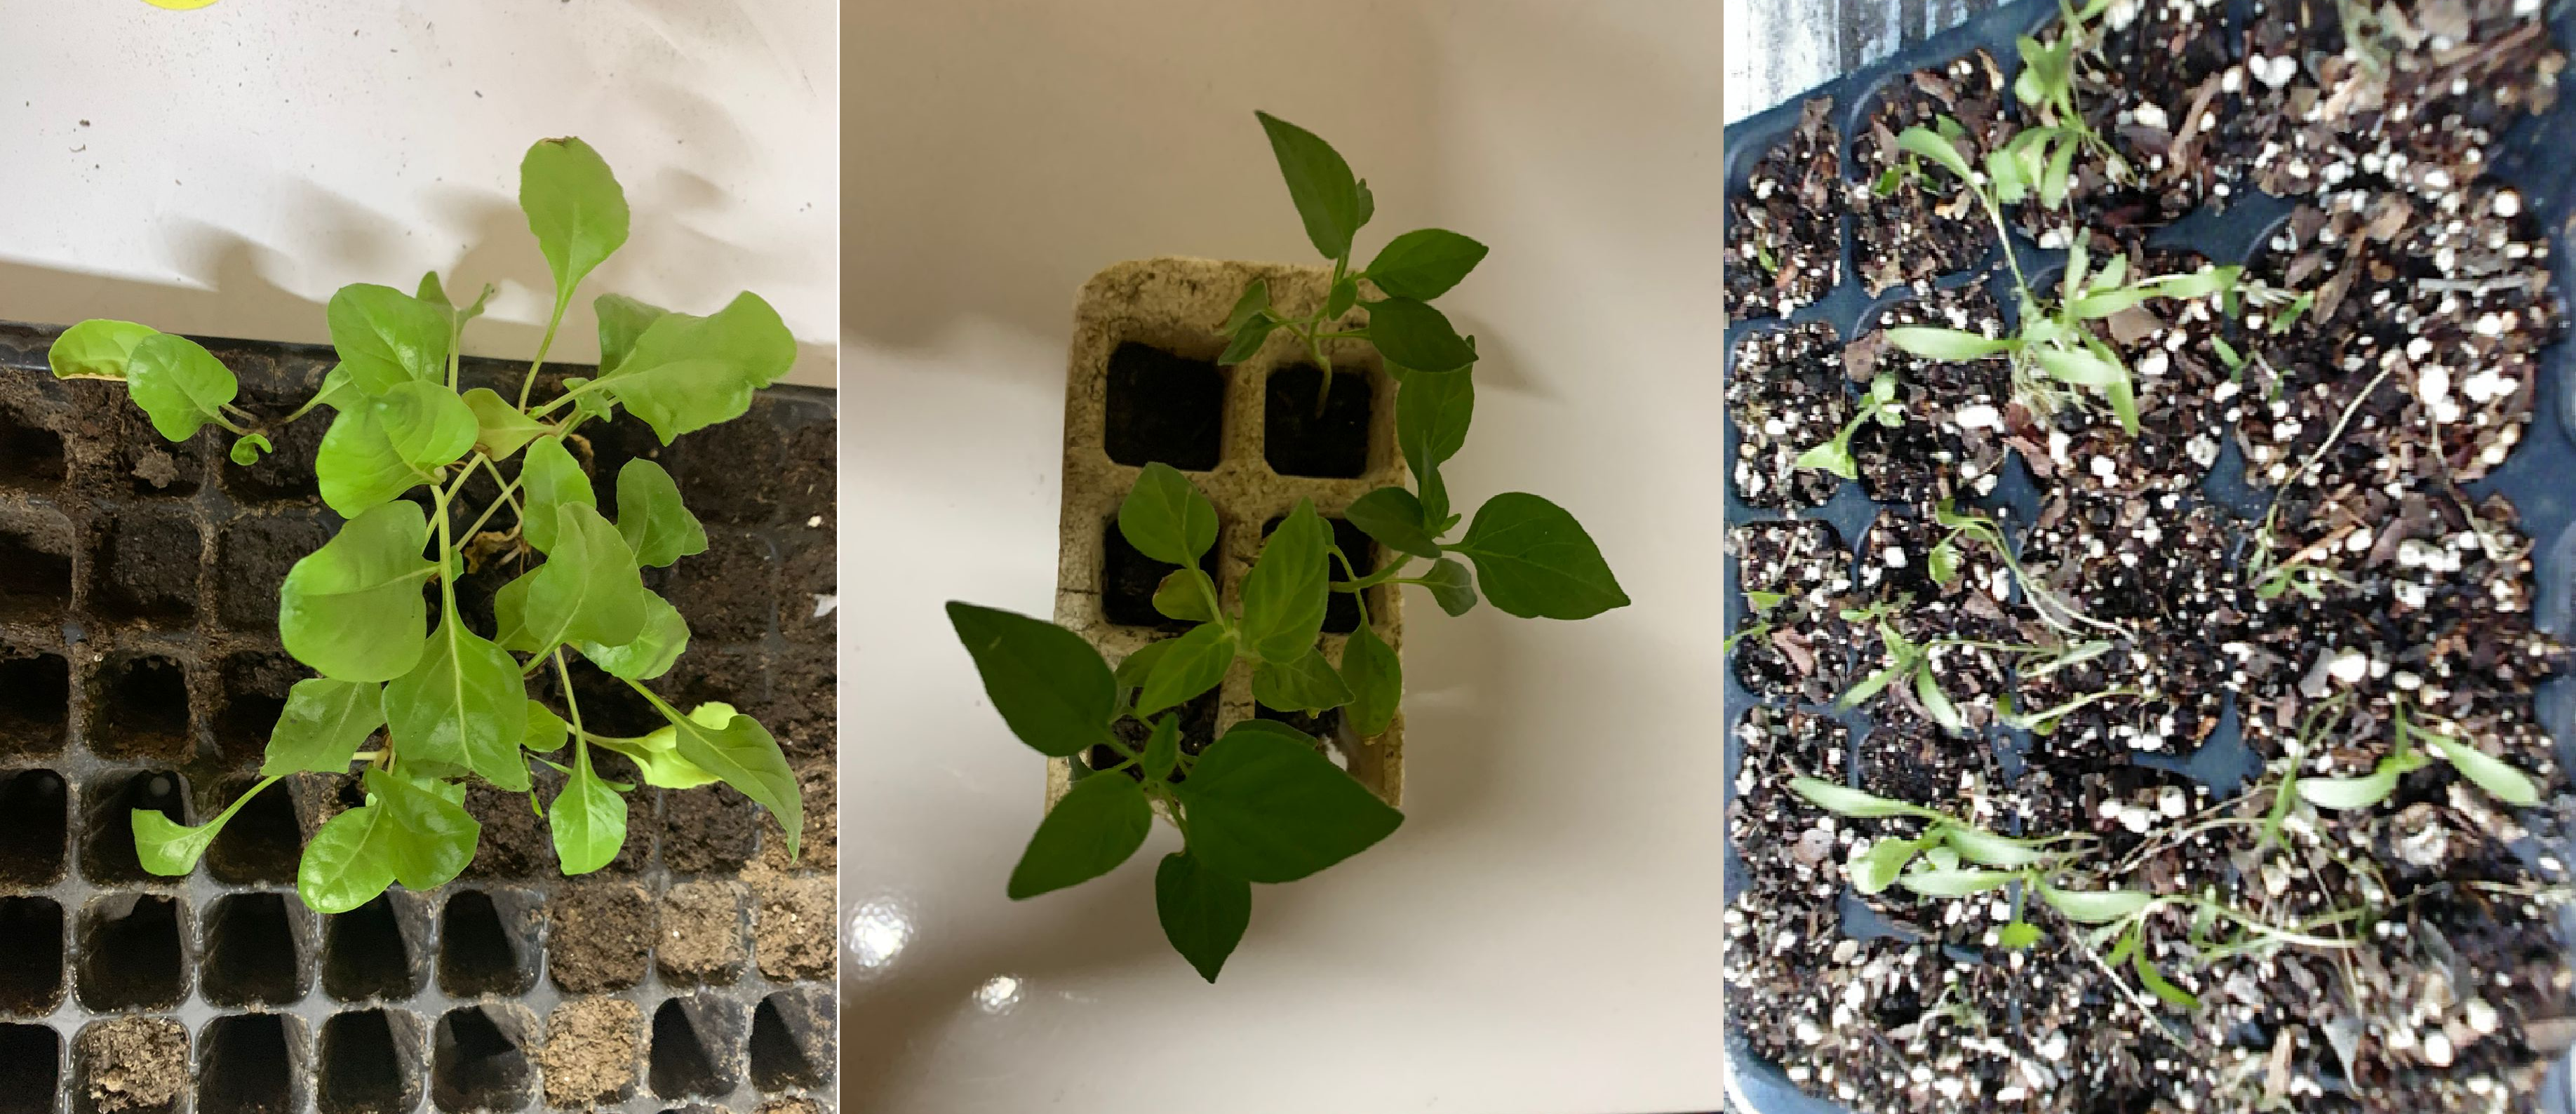
\includegraphics[scale=0.12]{imgs/plantas.png} \\
    \caption{Germinación de las plantas.}\label{plantas}
\end{figure}

\subsection{Visión por computadora}
Para el monitoreo de la germinación se programó un \textit{script} en el lenguaje de programación Python y la biblioteca OpenCV. La captura de video en tiempo real se realizó mediante una cámara web colocada sobre los semilleros con la ayuda de un tripié. La figura \ref{flujoseg} muestra el diagrama de flujo que resume las operaciones aplicadas sobre cada cuadro del video capturado para segmentar las zonas correspondientes a las plantas. Esta segmentación permitirá monitorear de manera automática el proceso de germinación de las plantas.

%\begin{itemize}
 %   \item Primeramente, se abre el ciclo de toma de video y para un mejor manejo del video se optó en convertir el espacio de color BGR a un espacio de color HSV, ya que es más fácil de trabajar en vez del espacio de color BGR. 
  %  \item Se define el rango de color que deseas segmentar, en nuestro caso pigmentos de color verde, por ende se define en función del espacio de color HSV. 
   % \item Se aplica una máscara a la toma de video original. 
    %\item Se muestra la toma original, la binarización y la segmentación del color verde.
    %\item Se realizan capturas cada día para observar el crecimiento de las plantas.
%\end{itemize}
 \begin{figure}[H]
\centering
         \includegraphics[scale=0.65]{imgs/FlujoSeg4.png} \\
    \caption{Diagrama de flujo para la segmentación de pigmentos verdes.}\label{flujoseg}
\end{figure}

%%%%%%%%%%%%%%%%%%%%%%%%%%%%%%%%%%%%%%%%%%%%%%%%%%%%%%%%%%%%%%%%%%%%%%%%%%%%%%%%%%%%%%%%%%%%%%%%%%%